% !TeX root = ActuarialFormSheet_MBFA-en.tex
% !TeX spellcheck = en_GB

\begin{f}[Pythagoras]
In a right triangle, the square of the hypotenuse is equal to the sum of the squares of the other two sides. If $ABC$ is right-angled at $C$, then

%
\begin{tikzpicture}[scale=.85]
	% Triangle
	\coordinate [label=above left:$C$] (C) at (0,0);
	\coordinate [label=above right:$B$] (B) at (4,0);
	\coordinate [label=below left:$A$] (A) at (0,3);
	
	%\draw[thick] (A) -- (B) -- (C) -- cycle;
	
	% Carré sur AC
	\draw[BleuProfondIRA!60] (A) -- (C) ;
	\node at (-0.6,1.5) {\color{BleuProfondIRA}$AC^2$};
	
	% Carré sur BC
	\draw[VertIRA] (B) -- (C);
	\node at (2,0.6) {\color{VertIRA}$BC^2$};
	
	% Carré sur AB
	\draw[OrangeProfondIRA] (A) -- (B) ;
	\node at (2.5,1.75) {\color{OrangeProfondIRA}$AB^2$};
	
	% Angle droit
	\draw (C) rectangle +(0.3,0.3);
	\node[right] at (3.75,1.75) {$
		\color{OrangeProfondIRA}AB^2 = \color{VertIRA}AC^2 +\color{BleuProfondIRA} BC^2
		$};
\end{tikzpicture}
\end{f}

\begin{f}[Thales]
Let two lines \textbf{intersect at a point} \( A \), and let two lines \( (BC) \) and \( (DE) \) \textbf{parallel}, intersecting the two lines at \( B, D \) and \( C, E \), then :
\[
\frac{AB}{AD} = \frac{AC}{AE} = \frac{BC}{DE}
\]


\begin{center}
	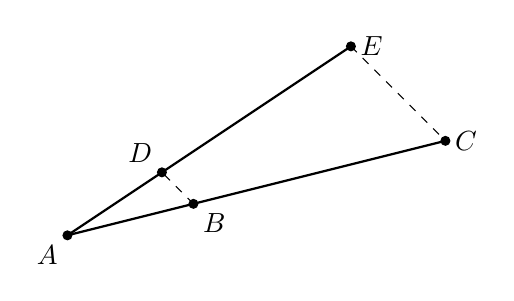
\begin{tikzpicture}[scale=.8]
		% Points
		\coordinate (A) at (0,0);
		\coordinate (B) at (2,0.5);
		\coordinate (C) at (6,1.5);
		\coordinate (D) at (1.5,1);
		\coordinate (E) at (4.5,3);
		
		% Segments
		\draw[thick] (A) -- (C);
		\draw[thick] (A) -- (E);
%		\draw[thick] (B) -- (C);
%		\draw[thick] (D) -- (E);
		\draw[dashed] (B) -- (D);
		\draw[dashed] (E) -- (C);
		
		% Points
		\filldraw[black] (A) circle (2pt) node[below left] {\(A\)};
		\filldraw[black] (B) circle (2pt) node[below right] {\(B\)};
		\filldraw[black] (C) circle (2pt) node[right] {\(C\)};
		\filldraw[black] (D) circle (2pt) node[above left] {\(D\)};
		\filldraw[black] (E) circle (2pt) node[right] {\(E\)};
		
%		% Parallèles
%		\draw[<->,blue,thick] (0.8,2.2) -- (3.2,2.2) node[right] {\small $\ell$};
%		\draw[<->,blue,thick] (0.8,0.8) -- (3.2,0.8) node[right] {\small $\ell'$};
%		\node at (3.6,1.5) {\small $\ell \parallel \ell'$};
	\end{tikzpicture}
\end{center}
\end{f}
\hrule

\begin{f} [Quadratic equation] 
     \[
    ax^2 + bx + c = 0
    \]

    The discriminant is defined by :
    
    \[
    \Delta = b^2 - 4ac
    \]
       
    \begin{itemize}
        \item If \(\Delta > 0\), the equation has two distinct solutions :
        \[
        x_1 = \frac{-b + \sqrt{\Delta}}{2a}, \quad x_2 = \frac{-b - \sqrt{\Delta}}{2a}
        \]
        \item If \(\Delta = 0\), the equation has a double solution :
        \[
        x = \frac{-b}{2a}
        \]
        \item If \(\Delta < 0\), the equation has a solution in the imaginary
        \[
        x_1 = \frac{-b + i\sqrt{\Delta}}{2a}, \quad x_2 = \frac{-b - i\sqrt{\Delta}}{2a}
        \]
    \end{itemize}
\end{f}
\hrule
\begin{f} [Factorial, Counting and Gamma Functions] 

The \textbf{factorial} function (of $\mathbb{N}$ in $\mathbb{N}$ ) is defined by $0!=1$ and $n!=n \times(n-1) \times \cdots \times 2 \times 1=$ permutations of $n$ elements $\displaystyle C_n^k=\binom{k}{n}=\frac{n!}{k!(n-k)!}=$ choice of $k$ elements among $n$ the $C_n^k$ are also calculated by Pascal's triangle and verify:

$$
C_n^k=C_n^{n-k}, C_n^k+C_n^{k+1}=C_{n+1}^{k+1} .
$$


Let $E$ be a set of cardinal $\operatorname{Card}(E)$ and parts $\mathcal{P}(E)$ :

$$
\begin{aligned}
\operatorname{Card}(\mathcal{P}(E)) & =2^{\operatorname{Card}(E)} \\
\operatorname{Card}(A \times B) & =\operatorname{Card}(A) \times \operatorname{Card}(B) \\
\operatorname{Card}(A \cup B) & =\operatorname{Card}(A)+\operatorname{Card}(B)-\operatorname{Card}(A \cap B)
\end{aligned}
$$
\[ \Gamma(n) = \int_0^\infty t^{n-1} e^{-t} \, dt \]
The function $\Gamma$ can be seen as the extension of the factorial : $\Gamma(n+1)=n!$.
\end{f}

\hrule
\begin{f}
	[Binomial expansion] 
	
	For a positive integer $n$,
	$$
	(x+y)^n=\sum_{i=0}^n\binom{n}{i} x^i y^{n-i}
	$$
	
\end{f}
\hrule
\begin{f}[Sequences]  
	
	Arithmetic sequences of reason $r$
	
	$$
	\left\{\begin{array} { r l } 
		{ u _ { n + 1 } } & { = u _ { n } + r } \\
		{ u _ { 0 } } & { \in \mathbb { R } }
	\end{array} \Rightarrow \left\{\begin{array}{rl}
		u_n & =n r+u_0 \\
		\sum_{k=0}^n u_k & =\frac{(n+1)\left(2 u_0+n r\right)}{2}
	\end{array}\right.\right.
	$$
	
	geometric sequences of reason $q\left\{\begin{array}{rll}u_{n+1} & = & q \times u_n \\ u_0 & \in & \mathbb{R}\end{array}\right.$
	
	$$
	\Rightarrow\left\{\begin{array}{rlr}
		u_n & =u_0 \times q^n \\
		\sum_{k=0}^n u_k & =\left\{\begin{array}{rl}
			(n+1) u_0 & \text { if } \\
			u_0 \frac{1-q^{n+1}}{1-q} & \text { otherwise }
		\end{array} \quad q=1\right.
	\end{array}\right.
	$$
	
\end{f}
\hrule
\begin{f}[Exponential and Logarithm]
	The exponential function \( e^x \) can be defined by the following power series expansion :
	
	\[
	e^x = \sum_{n=0}^{\infty} \frac{x^n}{n!} = 1 + x + \frac{x^2}{2!} + \frac{x^3}{3!} + \cdots
	\]
	
	This series converges for all \( x \in \mathbb{R} \) and allows us to define the exponential as an infinite sum.
	
	
	The natural logarithm function \( \ln(x) \) is defined as the antiderivative of the function \( \frac{1}{x} \). In other words :
	
	\[
	\frac{d}{dx} \ln(x) = \frac{1}{x}
	\]
	
	with the condition \( \ln(1) = 0 \). This definition allows us to establish the link between the exponential and the logarithm via inversion : \( e^{\ln(x)} = x \) for \( x > 0 \).
	
\end{f}



\hrule
\begin{f}[Congruence relationship]
	Let $m > 0$. We say that two real numbers $a$ and $b$ are congruent modulo $m$ if there exists a relative integer $k \in \mathbb{Z}$ such that :
	\[
	a = b + km.
	\]
	On note $a \equiv b \pmod{m}$.
	
	In trigonometry, we often choose $m = 2\pi$ or $m = \pi$.
\end{f}

\begin{f}
	[Trigonometric circle — sine, cosine, tangent]
	
		\begin{animateinline}[poster=first, autoplay,loop]{1}
			\multiframe{24}{i=0+1}{%
				\begin{tikzpicture}[scale=3,yrange=-4:4]
\node[text width=9cm, align=left] at (0,3.75) {\ $\displaystyle M = (\cos \theta, \sin \theta)$};
\node[text width=9cm, align=left] at (0,3.5) {\ If $\theta \not\equiv \frac{\pi}{2} \pmod{\pi}$, we define :
	$\displaystyle
	\tan \theta = \frac{\sin \theta}{\cos \theta}
	$};
\node[text width=9cm, align=left] at (0,3.25) {\ $\displaystyle \cos^2 \theta + \sin^2 \theta = 1 $};
\node[text width=9cm, align=left] at (0,2.5) {\renewcommand{\arraystretch}{1.5}\begin{tabular}{|c|c|c|c|c|c|}
		\hline\rowcolor{BleuProfondIRA!40}
		$\theta$ & $0$ & $\frac{\pi}{6}$ & $\frac{\pi}{4}$ & $\frac{\pi}{3}$ & $\frac{\pi}{2}$ \\
		\hline
		$\cos \theta$ & $1$ & $\frac{\sqrt{3}}{2}$ & $\frac{\sqrt{2}}{2}$ & $\frac{1}{2}$ & $0$ \\
		\hline
		$\sin \theta$ & $0$ & $\frac{1}{2}$ & $\frac{\sqrt{2}}{2}$ & $\frac{\sqrt{3}}{2}$ & $1$ \\
		\hline
		$\tan \theta$ & $0$ & $\frac{\sqrt{3}}{3}$ & $1$ & $\sqrt{3}$ & indéfini \\
		\hline
\end{tabular}};
\node[text width=9cm, align=left] at (0,-2.75) {\small\renewcommand{\arraystretch}{1.5}	
\begin{tabular}{|c|c|c|}
	\hline\rowcolor{BleuProfondIRA!40}
	$-\theta$ & $\theta + \pi$ & $\pi - \theta$ \\
	\hline
	$\cos \theta$ & $-\cos \theta$ & $-\cos \theta$ \\
	\hline
	$-\sin \theta$ & $-\sin \theta$ & $\sin \theta$ \\
	\hline
	\hline\rowcolor{BleuProfondIRA!40}
	$\theta + 2\pi$ & $\frac{\pi}{2} - \theta$ & $\frac{\pi}{2} + \theta$ \\
	\hline
	$\cos \theta$ & $\sin \theta$ & $-\sin \theta$ \\
	\hline
	$\sin \theta$ & $\cos \theta$ & $\cos \theta$ \\
	\hline
\end{tabular}
 \\ \vspace{2mm}
\ $\cos x = \cos y \iff \begin{cases}
	x \equiv y \pmod{2\pi} \text{ or }\\ x \equiv -y \pmod{2\pi}
\end{cases} $ \\
\ $\sin x = \sin y \iff \begin{cases}
	 x \equiv y \pmod{2\pi} \text{ or }\\ x \equiv \pi - y \pmod{2\pi}
\end{cases}$\\
\ $\tan x = \tan y \iff x \equiv y \pmod{\pi}$
};


	\def\radius{1}
	\pgfmathsetmacro{\angle}{15*\i+45} % degr\'es
	\pgfmathsetmacro{\cosx}{cos(\angle)}
	\pgfmathsetmacro{\siny}{sin(\angle)}
	
	% Coordonn\'ees de M
	\coordinate (M) at ({\cosx}, {\siny});
	
	% Axes
	\draw[->] (-0.2,0) -- (1.25,0) node[anchor=west] {$x$};
	\draw[->] (0,-1.5) -- (0,1.25) node[anchor=south] {$y$};
	
	% Cercle
	\draw[thick] (0,0) circle(\radius);
	
	% OM
	\draw[->, thick, BleuProfondIRA] (0,0) -- (M) node[above right] {$M$};
	
	% Projections cosinus et sinus
	\draw[dashed] (M) -- ({\cosx}, 0);
	\draw[dashed] (M) -- (0, {\siny});
	
	\draw[<->, thick, OrangeProfondIRA] (0, -0.1) -- ({\cosx}, -0.1);
	\node[below, OrangeProfondIRA] at ({\cosx/2}, -0.1) {$\cos\theta$};
	
	\draw[<->, thick, VertIRA] (-0.1, 0) -- (-0.1, {\siny});
	\node[left, VertIRA] at (-0.1, {\siny/2}) {$\sin\theta$};
	
	% Angle
	\draw[->, FushiaIRA] (0.5,0) arc[start angle=0, end angle=\angle, radius=0.5];
	\node at (0.7,0.15) {$\theta$};
	
	% Tangente (affich\'ee sauf si angle = 90\textdegree{} ou 270\textdegree{})
	\pgfmathtruncatemacro{\angleInt}{\angle} % angle en entier
	\ifnum\angleInt=90
	\draw[dashed] (1,-4) -- (1,4);
	\node[right] at (1,1.3) {$x=1$};
	\else\ifnum\angleInt=270
	\draw[dashed] (1,-4) -- (1,4);
	\node[right] at (1,1.3) {$x=1$};
	\else
	\pgfmathsetmacro{\tany}{tan(\angle)}
	\draw[dashed, gray] (0,0) -- (1.05, {\tany*1.05});
	\draw[dashed] (1,-4) -- (1,4);
	\coordinate (T) at (1, {\tany});
	\draw[fill=black] (T) circle(0.015);
	\node[above right] at (T) {$T$};
	\node[below right] at (T) {$(1,\tan\theta)$};
	\node[right] at (1,1.3) {$x=1$};
	\fi\fi
\end{tikzpicture}
			}%
		\end{animateinline}
	
\end{f}
\renewcommand{\arraystretch}{1}

\columnbreak
\begin{f}
	[Properties of the congruence relation]
	
	Let $m > 0$ et $a, b, c, d \in \mathbb{R}$. Then :
	
	\begin{itemize}
		\item \textbf{Reflexivity} : $a \equiv a \pmod{m}$.
		\item \textbf{Symmetry} : $a \equiv b \pmod{m} \iff b \equiv a \pmod{m}$.
		\item \textbf{Transitivity} : if $a \equiv b \pmod{m}$ and $b \equiv c \pmod{m}$, then $a \equiv c \pmod{m}$.
		\item \textbf{Additivity} : if $a \equiv b \pmod{m}$ and $c \equiv d \pmod{m}$, then $a + c \equiv b + d \pmod{m}$.
	\end{itemize}
	
\end{f}	

\hrule
\begin{f}[Derivatives and primitives] 

\[
\begin{aligned}
& f \text { continues in } x_\mathrm{m} \Leftrightarrow \lim _{x \rightarrow x_\mathrm{m}} f(x)=f\left(x_\mathrm{m}\right) \\
& f \text { derivable in } x_\mathrm{m} \Leftrightarrow \exists \lim _{h \rightarrow 0} \frac{f\left(x_\mathrm{m}+h\right)-f\left(x_\mathrm{m}\right)}{h}=: f^{\prime}\left(x_\mathrm{m}\right)
\end{aligned}
\]
 
The \textbf{Riemann integral} of a function \(f(x)\) on an interval \([a, b]\) is the limit, if it exists, of the sum of the areas of the rectangles approaching the area under the curve, given by :  

\[
\int_a^b f(x) \, dx = \lim_{n \to \infty} \sum_{i=1}^n f(x_i^*) \Delta x_i,
\]
\begin{itemize}
\item \( [x_{i-1}, x_i] \) is a subdivision of \([a, b]\),  
\item \( \Delta x_i = x_i - x_{i-1} \) is the width of the subinterval,  
\item \( x_i^* \in [x_{i-1}, x_i] \) is an arbitrarily chosen point in each subinterval.
\end{itemize}
  
\newcounter{numberofdiscretisation} \setcounter{numberofdiscretisation}{1}
\begin{center}
	    \begin{animateinline}[autoplay,loop,poster=15]{2}
      \whiledo{\thenumberofdiscretisation<20}{
        \begin{tikzpicture}[line cap=round, line join=round, >=triangle 45,
                            x=2.6cm, y=1.0cm, scale=1]
           \draw [->,color=OrangeProfondIRA] (-0.1,0) -- (2.5,0);
          \foreach \x in {1,2}
            \draw [shift={(\x,0)}, color=OrangeProfondIRA] (0pt,2pt)
                  -- (0pt,-2pt) node [below] {\footnotesize $\x$};
          \draw [color=OrangeProfondIRA] (2.5,0) node [below] {$x$};
          \draw [->,color=OrangeProfondIRA] (0,-0.1) -- (0,4.5);
          \foreach \y in {1,2,3,4}
            \draw [shift={(0,\y)}, color=OrangeProfondIRA] (2pt,0pt)
                  -- (-2pt,0pt) node[left] {\footnotesize $\y$};
          \draw [color=OrangeProfondIRA] (0,4.5) node [right] {$y$};
          \draw [color=OrangeProfondIRA] (0pt,-10pt) node [left] {\footnotesize $0$};
          \draw [color=OrangeProfondIRA, domain=0:2.2, line width=1.0pt] plot (\x,{(\x)^2});
          \clip(0,-0.5) rectangle (3,5);
          \draw (2,0) -- (2,4);
          \foreach \i in {1,...,\thenumberofdiscretisation}
            \draw [draw=BleuProfondIRA,fill=BleuProfondIRA,fill opacity=0.3, smooth,samples=50] ({1+(\i-1)/\thenumberofdiscretisation},{(1+(\i)/\thenumberofdiscretisation)^2})
                  --({1+(\i)/\thenumberofdiscretisation},{(1+(\i)/\thenumberofdiscretisation)^2})
                  --  ({1+(\i)/\thenumberofdiscretisation},0)
                  -- ({1+(\i-1)/\thenumberofdiscretisation},0)
                  -- cycle;
        \end{tikzpicture}
        %
        \stepcounter{numberofdiscretisation}
        \ifthenelse{\thenumberofdiscretisation<20}{ \newframe }{\end{animateinline} }
      }
      
\end{center}
      Example of a Riemann integral (upper)\href{https://texample.net/media/tikz/examples/TEX/upper-riemann-sum.tex}{$^*$}
 
 

The \textbf{Lebesgue integral} of a function \( f(x) \) on a set \( E \) is defined by measuring the area under the curve as a function of the values taken by \( f \), given by :  
\[
\int_E f \, d\mu = \int_0^\infty \mu(\{x \in E : f(x) > t\}) \, dt,
\]
\begin{itemize}
    \item \( \mu \) is a measure (often the Lebesgue measure),  
\item \( \{x \in E : f(x) > t\} \) represents the set of points where \( f(x) \) exceeds \( t \).  
\end{itemize} 
Unlike Riemann, Lebesgue groups points according to their values rather than their position.

\renewcommand{\arraystretch}{1.5}
\[
\begin{array}{|c|c|c|}
\hline \rowcolor{BleuProfondIRA!40} \text { function }(n \in \mathbb{R}) & \text { derivative } & \text { primitive } \\
\hline x & 1 & \frac{x^2}{2}+C \\
\hline x^2 & 2 x & \frac{x^3}{3}+C \\
\hline 1 / x & -1 / x^2 & \ln (x)+C \\
\hline \sqrt{x}=x^{1 / 2} & \frac{1}{2 \sqrt{x}} & \frac{2}{3} x^{3 / 2}+C \\
\hline x^n, n \neq-1 & n x^{n-1} & \frac{x^{n+1}}{n+1}+C \\
\hline \ln (x) & 1 / x & x \ln (x)-x+C \\
\hline e^x & e^x & e^x+C \\
\hline a^x=e^{x \ln (a)} & \ln (a) \times a^x & a^x / \ln (a)+C \\
\hline \sin (x) & \cos (x) & -\cos (x)+C \\
\hline \cos (x) & -\sin (x) & \sin (x)+C \\
\hline \tan (x) & 1+\tan (x) & -\ln (|\cos (x)|)+C \\
\hline 1 /\left(1+x^2\right) & -2 x /\left(1+x^2\right)^2 & \arctan (x)+C \\
\hline
\end{array}
\]
\renewcommand{\arraystretch}{1}

\[
    \begin{array}{rl|rl}
(u+v)^{\prime} & =u^{\prime}+v^{\prime} & \left(\frac{1}{u}\right)^{\prime} & =-\frac{u^{\prime}}{u^2} \\
(k u)^{\prime} & =k u^{\prime} & (\ln (u))^{\prime} & =\frac{u^{\prime}}{u} \\
(u \times v)^{\prime} & =u^{\prime} v+u v^{\prime} & (\exp (u))^{\prime} & =\exp (u) \times u^{\prime} \\
\left(\frac{u}{v}\right)^{\prime} & =\frac{u^{\prime} v-u v^{\prime}}{v^2} & (f(u))^{\prime} & =f^{\prime}(u) \times u^{\prime} \\
\left(u^n\right)^{\prime} & =n u^{n-1} \times u^{\prime} & (f \circ u)^{\prime} & =\left(f^{\prime} \circ u\right) \times u^{\prime}
\end{array}
\]
\end{f}

\hrule

\begin{f} [Integration by parts] 

Either \( u(x) \) et \( v(x) \) two continuously differentiable functions on the interval \([a, b]\), then

\[
\int_a^b u(x) v'(x) \, dx = \left[ u(x) v(x) \right]_a^b - \int_a^b u'(x) v(x) \, dx
\]

or :
\begin{itemize}
    \item \( u(x) \) is a function whose derivative is known \( u'(x) \),
    \item \( v'(x) \) is a function whose primitive is known \( v(x) \).
\end{itemize}

\end{f}
\hrule
\begin{f}[Integration with change of variable] 

Either \( f(x) \) a continuous function and \( x = \phi(t) \) a change of variable, where \( \phi \) is a differentiable function. Then :

\[
\int_{a}^{b} f(x) \, dx = \int_{\phi^{-1}(a)}^{\phi^{-1}(b)} f(\phi(t)) \phi'(t) \, dt
\]

or :
\begin{itemize}
    \item \( x = \phi(t) \) represents the change of variable,
    \item \( \phi'(t) \) is the derivative of \( \phi(t) \),
    \item the limits of the integral are adjusted according to the change of variable.
\end{itemize}
\end{f}

\hrule
\begin{f}
 [Taylor formula] 
 
Either \( f(x) \) a function \( n \) - times differentiable at a point \( a \). Taylor's development of \( f(x) \) around \( a \) is given by :

\begin{align*}
 f(x) =& f(a) + f'(a)(x - a) + \frac{f''(a)}{2!}(x - a)^2 \\
 &+ \cdots + \frac{f^{(n)}(a)}{n!}(x - a)^n + \mathcal{O}_n(x)
\end{align*}


où :
\begin{itemize}
    \item \( f^{(n)}(a) \) is the \( n \)\ieme{} derived from \( f \) evaluated in \( a \),
    \item \( \mathcal{O}_n(x) \) is the remainder of the Taylor development, representing the approximation error when truncating the series after the order term \( n \), then 
    \[
    \lim_{x\rightarrow 0}\frac{\mathcal{O}_n(x) }{x^n}\Rightarrow 0
    \]
\end{itemize}
\end{f}
\hrule
\begin{f}[Intermediate Value Theorem] 

Either \( f \) a continuous function on a closed interval \([a, b]\) and \( f(a) \neq f(b) \). The intermediate value theorem states that for any real number \( c \) between \( f(a) \) and \( f(b) \), there is a point \( x \in [a, b] \) such as :

\[
f(x) = c
\]

In other words, if a function is continuous on an interval, it takes all the values between \( f(a) \) and \( f(b) \) at least once.
\end{f}
\hrule
\begin{f}[Matrices and properties]
  
\textbf{Diagonal matrices :}
A matrix is said to be diagonal if all elements outside the main diagonal are zero. For a matrix \( A \in \mathbb{R}^{n \times n} \), it is written :
\[
A = \text{diag}(a_1, a_2, \dots, a_n)
\]
where \( a_i \) are the diagonal elements.

\textbf{Triangular matrices :}
A matrix is upper triangular if all elements below the diagonal are zero, that is, \( A_{ij} = 0 \) for \( i > j \). Conversely, it is lower triangular if \( A_{ij} = 0 \) for \( i < j \).
\end{f}
\begin{f}[Determinant of a matrix]
  
The determinant of a square matrix \( A \in \mathbb{R}^{n \times n} \) is a scalar, denoted \( \det(A) \) :
\begin{itemize}
    \item If \( A \) is a square matrix \( n \times n \), then \( A \) is invertible if and only if \( \det(A) \neq 0 \).
    \item The determinant of an upper or lower triangular matrix or a diagonal matrix :
    \[
    \det(A) = \prod_{i=1}^{n} A_{ii}
    \]
    \item
    \[
    \det(AB) = \det(A) \cdot \det(B),\quad \det(\lambda B) = \lambda\det(B), 
    \]
    \item 
    \[
    \det(A^T) = \det(A)
    \]
    \item If a matrix \( A \) contains two identical rows or columns, then \( \det(A) = 0 \).
\end{itemize}

\textbf{Calculation of the determinant :}
The determinant of a matrix \( 2 \times 2 \) is simply calculated by :
\[
\det\begin{pmatrix} a & b \\ c & d \end{pmatrix} = ad - bc
\]
For a matrix \( 3 \times 3 \), it is given by :
\[
\det\begin{pmatrix} a & b & c \\ d & e & f \\ g & h & i \end{pmatrix} = a(ei - fh) - b(di - fg) + c(dh - eg)
\]
For higher-dimensional matrices, the determinant can be calculated by cofactors or via a reduction method (e.g., Gauss's method).

\end{f}
\hrule
\begin{f}[Invertibility of a matrix] 
A matrix \( A \in \mathbb{R}^{n \times n} \) is invertible if there exists a matrix \( A^{-1} \) such as :
\[
A A^{-1} = A^{-1} A = I_n
\]
or \( I_n \) is the identity matrix. The invertibility of a matrix is guaranteed by \( \det(A) \neq 0 \).

\textbf{Trace :}
The trace of a square matrix \( A \), noted \( \text{Tr}(A) \), is the sum of its diagonal elements :
\[
\text{Tr}(A) = \sum_{i=1}^{n} A_{ii}
\]
It often represents quantities linked to the sum of the eigenvalues of a matrix.

\textbf{Cholesky decomposition :}
Cholesky decomposition is applicable to positive definite symmetric matrices. It allows a matrix to be factorized \( A \in \mathbb{R}^{n \times n} \) into a product of the form :
\[
A = LL^T
\]
or \( L \) is a lower triangular matrix. This decomposition is useful in numerical calculations and optimization algorithms.

\end{f}
\hrule

\begin{f}[Gradient and Hessian matrix]
	For a function \( f : \mathbb{R}^n \rightarrow \mathbb{R} \) of class \( C^2 \), we define :
	
	\begin{itemize}
		\item The \textbf{gradient} \( \nabla f(x) \) as the vector of first partial derivatives :
		$$
		\nabla f(x) = 
		\begin{pmatrix}
			\frac{\partial f}{\partial x_1}(x) \\
			\vdots \\
			\frac{\partial f}{\partial x_n}(x)
		\end{pmatrix}
		$$
		
		\item The \textbf{Hessian matrix} \( \nabla^2 f(x) \) as the symmetric matrix of second derivatives :
		$$
		\nabla^2 f(x) =
		\begin{pmatrix}
			\frac{\partial^2 f}{\partial x_1^2}(x) & \cdots & \frac{\partial^2 f}{\partial x_1 \partial x_n}(x) \\
			\vdots & \ddots & \vdots \\
			\frac{\partial^2 f}{\partial x_n \partial x_1}(x) & \cdots & \frac{\partial^2 f}{\partial x_n^2}(x)
		\end{pmatrix}
		$$
	\end{itemize}
	
\end{f}

\begin{f}[Implicit Function Theorem]
	Either \( F : \mathbb{R}^2 \rightarrow \mathbb{R} \) a class function \( C^1 \), and suppose that \( F(a^\star, b) = 0 \) for a certain couple \( (a^\star, b) \in \mathbb{R}^2 \). If
	\[
	\frac{\partial F}{\partial y}(a^\star, b) \neq 0,
	\]
	so there is a real \( h > 0 \) and a single function \( \varphi \), defined on a neighbourhood \( (a^\star - h, a^\star + h) \), such as
	\[
	\varphi(a^\star) = b \quad \text{et} \quad \forall x \in (a^\star - h, a^\star + h), \quad F(x, \varphi(x)) = 0
	\]
	
	In addition, the implicit function \( \varphi \) is of class \( C^1 \) and its derivative is given by :
	\[
	\varphi'(x) = - \left. \frac{\partial F / \partial x}{\partial F / \partial y} \right|_{y = \varphi(x)}
	\]
	

\end{f}
